\documentclass[12pt]{article}


\usepackage{arxiv}
\usepackage[utf8]{inputenc} 	% allow utf-8 input
\usepackage[T1]{fontenc}    	% use 8-bit T1 fonts
\usepackage{hyperref}       	% hyperlinks
\usepackage{url}            		% simple URL typesetting
\usepackage{booktabs}       	% professional-quality tables
\usepackage{amsfonts}       	% blackboard math symbols
\usepackage{nicefrac}       	% compact symbols for 1/2, etc.
\usepackage{microtype}      	% microtypography
\usepackage{cite}
\usepackage{array}
\usepackage{multirow}
\usepackage{graphicx}
\usepackage{subcaption}
\usepackage{float}
\usepackage{tikz}
\usepackage{setspace}
\usetikzlibrary{matrix}
\usepackage{xspace}
\usepackage{extsizes}
%\doublespace

\usepackage{listings}
\usepackage{color}


\definecolor{dkgreen}{rgb}{0,0.6,0}
\definecolor{gray}{rgb}{0.5,0.5,0.5}
\definecolor{mauve}{rgb}{0.58,0,0.82}


\lstset{frame=tb,
language=Python,
aboveskip=3mm,
belowskip=3mm,
showstringspaces=false,
columns=flexible,
basicstyle={\small\ttfamily},
numbers=none,
numberstyle=\tiny\color{gray},
keywordstyle=\color{blue},
commentstyle=\color{dkgreen},
stringstyle=\color{mauve},
breaklines=true,
breakatwhitespace=true,
tabsize=3
}

\renewcommand\part[1]{\vspace{.10in}\textbf{#1}\par}

\title{Final Project}


\author{
Eric Altenburg\\
\And
David Horowitz\\
\And
Lachlan Mountjoy\\
}



\begin{document}


\maketitle

\begin{center}
	\textit{Pledge: I pledge my honor that I have abided by the Stevens Honor System.}
\end{center}

% keywords can be removed
%\keywords{Unmanned Aerial Vehicle \and UAV \and Drone \and Battery \and Battery Consumption \and Battery Usage \and Predict}

\section{Report}
	\begin{doublespace}
	\subsection{Executive Summary}
		We are a group of students at Stevens Institute of Technology interested in statistics and its real world applications. We are analyzing how the flavor of cheese can be altered by several different chemicals found in the cheese. Our previous research into chemical compounds lead us to the idea that acetic acid, hydrogen sulfide, and lactic acid could be major contributors to the flavor of cheese. Those are the variables we explore in this research. We believe that studying what causes a cheese to taste better could allow us to develop more flavorful and marketable cheeses.\par
	
	\subsection{Data Set}
		Our data set contains 30 different measurements from a set of cheddar cheeses. The variables being measured result from chemical processes which occur when cheddar cheese matures. The cheese is from the LaTrobe Valley of Victoria in Victoria, Australia. “Taste” is the main response variable being explored which is related to the concentrations of various chemicals in the cheese. The taste values were measured by combining the taste rankings from several different participants. Three explanatory variables were measured and recorded from the cheese: acetic acid, hydrogen sulfide (H2S), and lactic acid. For acetic acid and hydrogen sulfide, logarithmic transformations were taken. Lactic acid did not have a logarithmic transformation. The variable “Case” corresponds to the observation number 1 to 30. \par
		
	\subsection{Software}
		We used the R programming language combined with the RStudio development environment. We used the base packages included with R for our analysis. We also used \LaTeX \xspace to create the document.\par
		
	\subsection{Analysis}
		Our analysis is broken down into several components. We began with an overview of the data. This broad analysis shows the general statistics of the data such as the mean, standard deviation, and quartile ranges.\par
	\begin{center}
	\begin{tabular}{lcccc}
		& Mean & Median & St. Dev. & IQR\\
		Taste & 24.53 & 20.93 & 16.26 & 23.15\\
		Acetic & 5.50 & 5.42 & 0.57 & 0.646\\
		H2S & 5.94 & 5.33 & 2.13 & 3.597\\
		Lactic & 1.44 & 1.45 & 0.3 & 0.417\\
	\end{tabular}
	\end{center}\par
		We calculated the correlations between each combination of variables, this gave us a good starting point as to which variables might be related and told us which multiple regressions would be the best. \par
	\begin{center}
	\begin{tabular}{lcccc}
		& Taste & Acetic & H2S & Lactic\\
		Taste & 1.0000000 & 0.5495393 & 0.7557523 & 0.7042362\\
		Acetic & 0.5495393 & 1.0000000 & 0.6179559 & 0.6037826\\
		H2S & 0.7557523 & 0.6179559 & 1.0000000 & 0.6448123\\
		Lactic & 0.7042362 & 0.6037826 & 0.6448123 & 1.0000000\\
	\end{tabular}
	\end{center}\par
		We also ran 3 linear regressions on the dataset to find whether or not the explanatory variables are linearly related. \par
	\begin{center}
	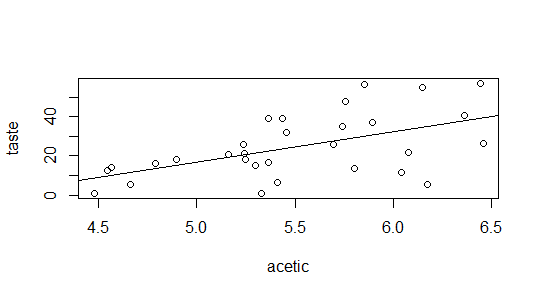
\includegraphics[width=.5\textwidth, height=60mm, keepaspectratio]{images/1155/1155_acetic_taste_linreg.png}\par
	\begin{tabular}{ccc}
		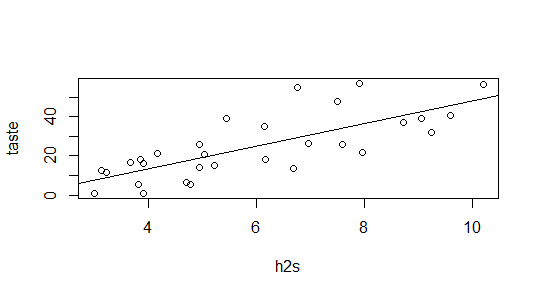
\includegraphics[width=.5\textwidth, height=60mm, keepaspectratio]{images/1156/h2s_taste_linear_regression.png}\par & 	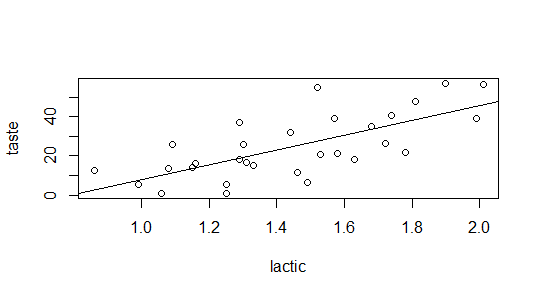
\includegraphics[width=.5\textwidth, height=60mm, keepaspectratio]{images/1157/taste_lactic_linear_regression.png}\par\\
	\end{tabular}
	\end{center}\par
		The residuals from each of the linear regressions are close to linear which indicates that our model is a good fit. Afterwards, we computed multiple linear regressions to see if they were better models than the single regressions were. We found that the model that used H2S and Lactic was the best in the end, due to its low P value in comparison to the other models. The remainder of the calculations and results can be found in the second section of the document.\par
	\end{doublespace}

\section{Data}
\part{11.53}
	\begin{center}
	\begin{tabular}{lcccc}
		& Mean & Median & St. Dev. & IQR\\
		Taste & 24.53 & 20.93 & 16.26 & 23.15\\
		Acetic & 5.50 & 5.42 & 0.57 & 0.646\\
		H2S & 5.94 & 5.33 & 2.13 & 3.597\\
		Lactic & 1.44 & 1.45 & 0.3 & 0.417\\
	\end{tabular}
	\end{center}\par
	\newpage
	Taste STEM: The decimal points 1 digit(s) to the right of the |\par
	\begin{tabular}{lcl}
		0 & | & 11666\\
		1 & | & 223456788\\
		2 & | & 112667\\
		3 & | & 25799\\
		4 & | & 18\\
		5 & | & 577\\
	\end{tabular}\par
	
	Acetic STEM: The decimal point is 1 digit(s) to the left of the |\par
	\begin{tabular}{lcl}
		44 & | & 846\\
		46 & | & 69\\
		48 & | & 0\\
		50 & | & 6\\
		52 & | & 4450377\\
		54 & | & 146\\
		56 & | & 046\\
		58 & | & 069\\
		60 & | & 4858\\
		62 & | & 7\\
		64 & | & 56\\
	\end{tabular}\par
	
	H2S STEM: The decimal point is at the |\par
	\begin{tabular}{lcl}
		2 & | & \\
		3 & | & 01278999\\
		4 & | & 27899\\
		5 & | & 024\\
		6 & | & 1728\\
		7 & | & 0569\\
		8 & | & 07\\
		9 & | & 126\\
		10 & | & 2\\
	\end{tabular}\par
	
	Lactic STEM: The decimal point is 1 digit(s) to the left of the |\par
	\begin{tabular}{lcl}
		8 & | & 69\\
		10 & | & 68956\\
		12 & | & 5599013\\
		14 & | & 4692378\\
		16 & | & 38248\\
		18 & | & 109\\
		20 & | & 1\\
	\end{tabular}\par
	
	\begin{center}
	\scalebox{0.9}{
	\begin{tabular}{cc}
	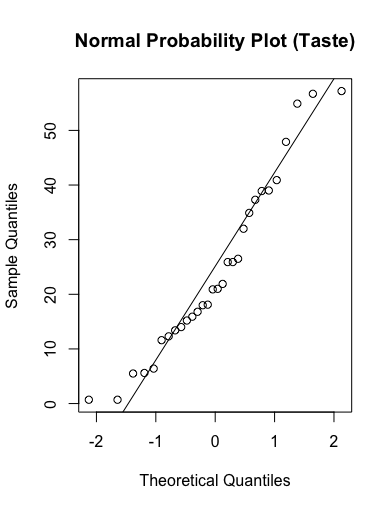
\includegraphics[width=.5\textwidth, keepaspectratio]{images/1153/normtaste.png} & 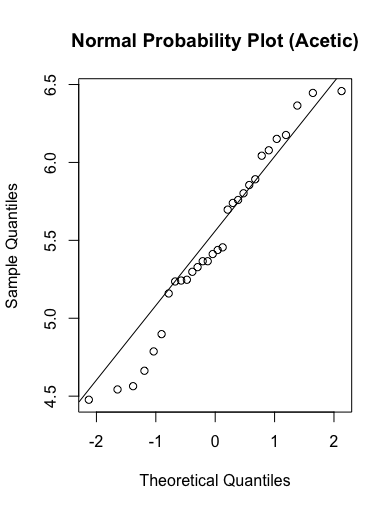
\includegraphics[width=.5\textwidth, keepaspectratio]{images/1153/normacetic.png}\\
	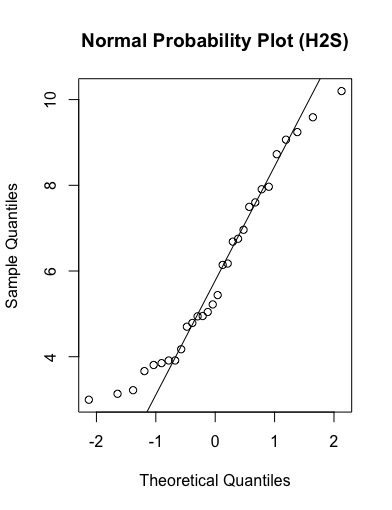
\includegraphics[width=.5\textwidth, keepaspectratio]{images/1153/normh2s.png} & 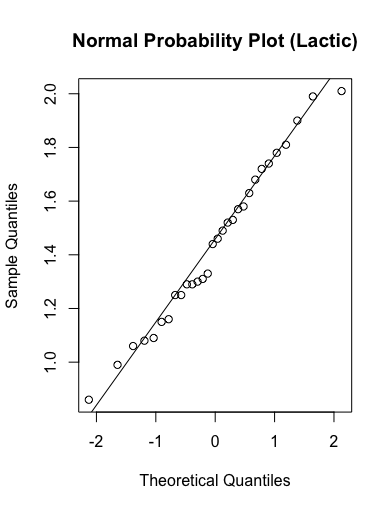
\includegraphics[width=.5\textwidth, keepaspectratio]{images/1153/normlactic.png}\\
	\end{tabular}}
	\end{center}\par
	All of the above plots showed normality among all data sites as the plotted observations were close to the line.\par
	
\newpage
\part{11.54} % can put in resize box
	%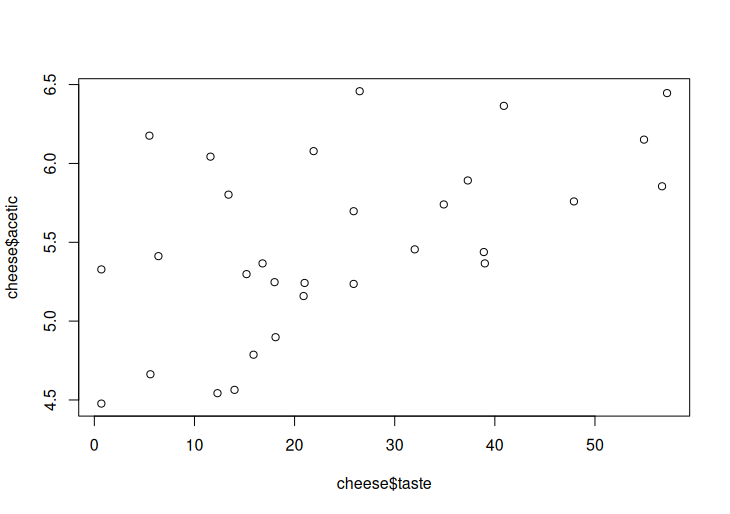
\includegraphics[width=.7\textwidth, keepaspectratio]{images/1154/1154graph1.png}
	\begin{center}
	\begin{tabular}{cc}
	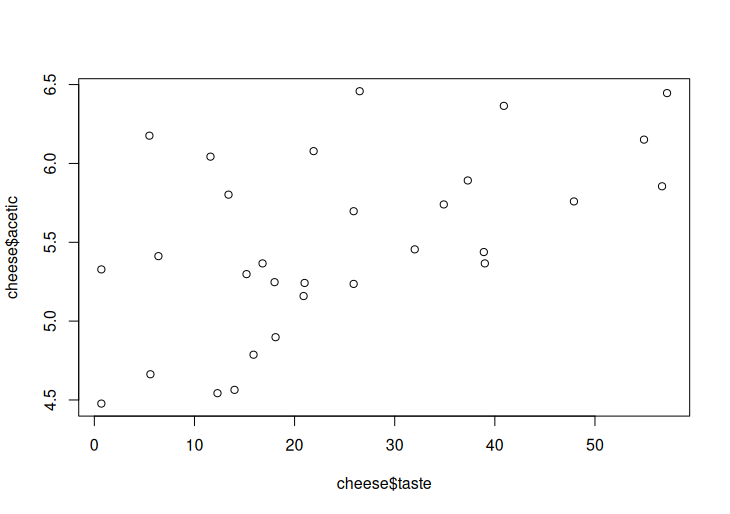
\includegraphics[width=.5\textwidth, height=60mm, keepaspectratio]{images/1154/1154graph1.png} & 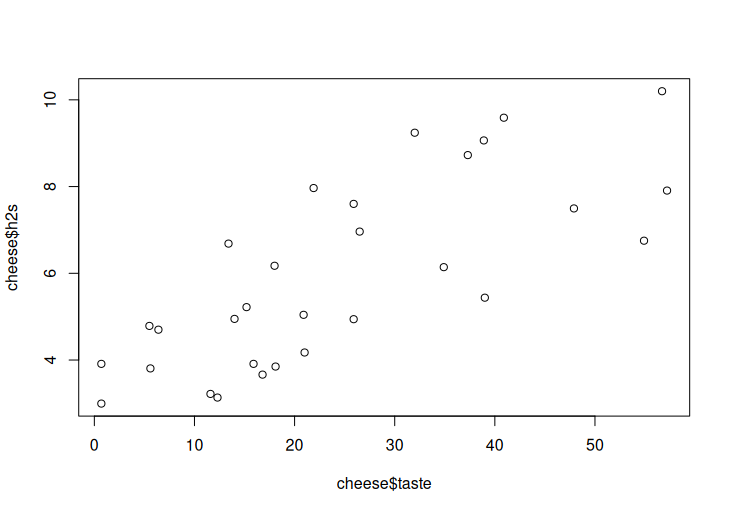
\includegraphics[width=.7\textwidth, height=60mm, keepaspectratio]{images/1154/1154graph2.png}\\
	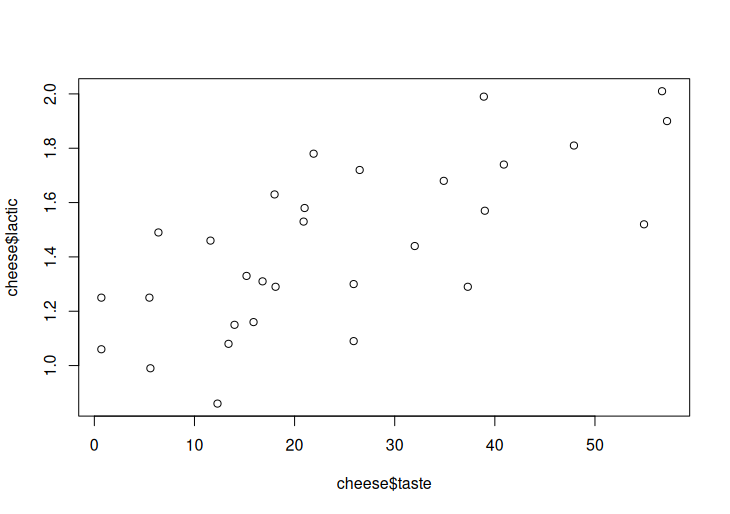
\includegraphics[width=.5\textwidth, height=60mm, keepaspectratio]{images/1154/1154graph3.png} & 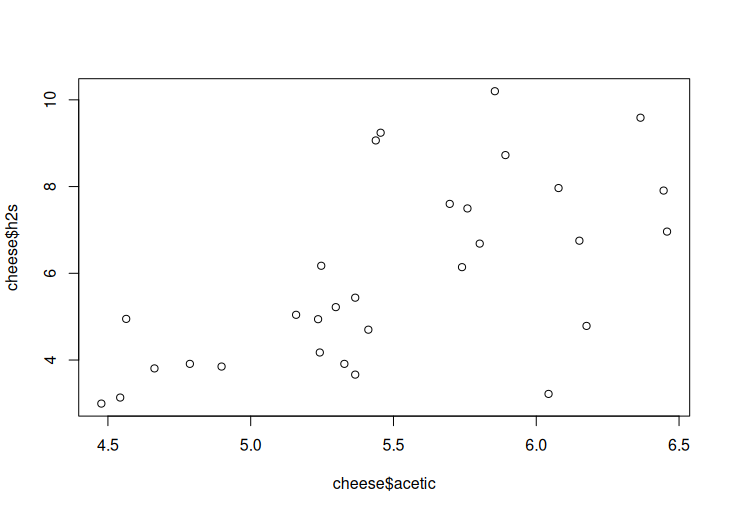
\includegraphics[width=.7\textwidth, height=60mm, keepaspectratio]{images/1154/1154graph4.png}\\
	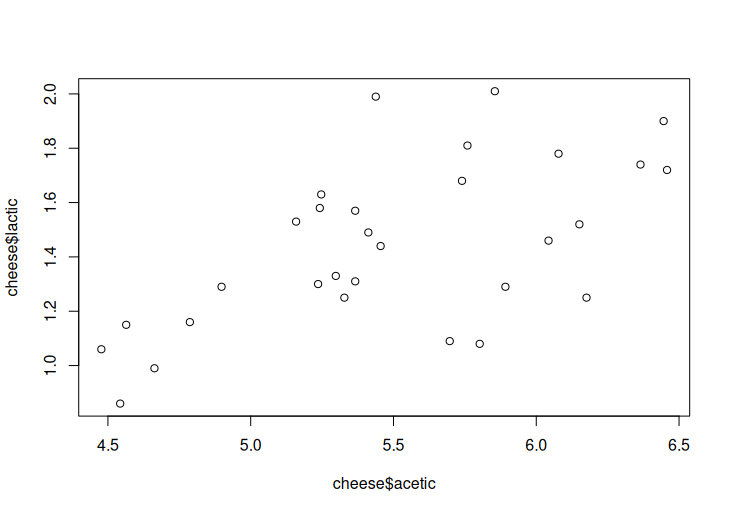
\includegraphics[width=.5\textwidth, height=60mm, keepaspectratio]{images/1154/1154graph5.png} & 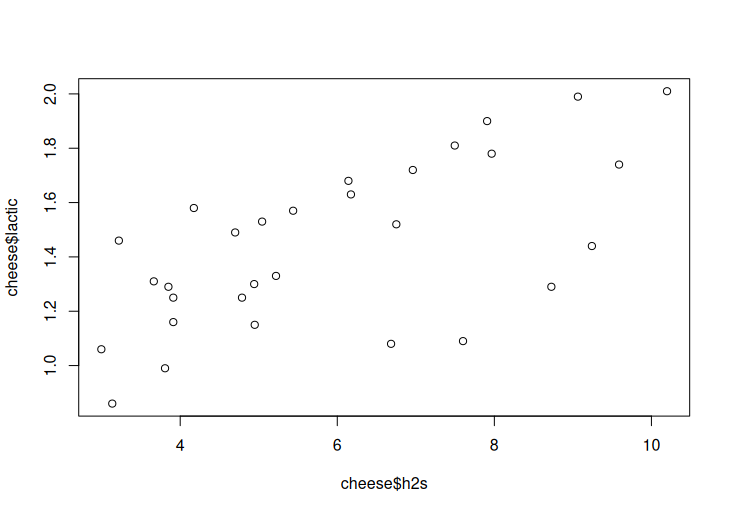
\includegraphics[width=.7\textwidth, height=60mm, keepaspectratio]{images/1154/1154graph6.png}\\
	\end{tabular}
	\end{center}\par
	For all the above graphs, the relationships are positive.\par
	
	\begin{tabular}{cc}
	Coorelation & P-value\\
	\begin{tabular}{lcccc}
		& Taste & Acetic & H2S & Lactic\\
		Taste & 1.0000000 & 0.5495393 & 0.7557523 & 0.7042362\\
		Acetic & 0.5495393 & 1.0000000 & 0.6179559 & 0.6037826\\
		H2S & 0.7557523 & 0.6179559 & 1.0000000 & 0.6448123\\
		Lactic & 0.7042362 & 0.6037826 & 0.6448123 & 1.0000000\\
	\end{tabular}
	& 
	\begin{tabular}{ll}
		Taste, Acetic & 0.001658192\\
		Taste, H2S & $1.373783*10^{-6}$\\
		Taste, Lactic & $1.405117*10^{-5}$\\
		Acetic, H2S & 0.0002739173\\
		Acetic, Lactic & 0.0004113657\\
		H2S, Lactic & 0.0001198401\\
	\end{tabular}
	\end{tabular}

\newpage
\part{11.55}
	%regression, residual, summary, other two
	\begin{center}
	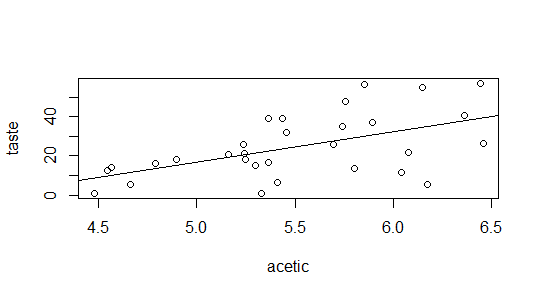
\includegraphics[width=.5\textwidth, height=60mm, keepaspectratio]{images/1155/1155_acetic_taste_linreg.png}\par
	
	Summary\par
	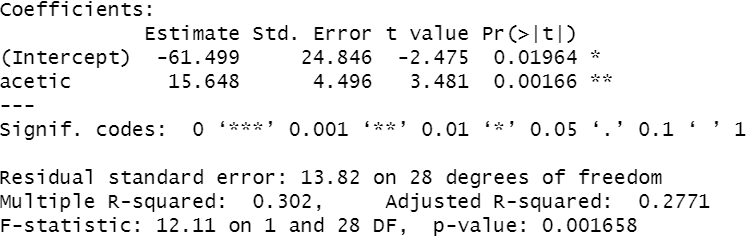
\includegraphics[width=.5\textwidth, height=60mm, keepaspectratio]{images/1155/1155_acetic_taste_summary.PNG}\par
	H$_{0}: \beta_{1} = 0$, Acetic and Taste are not related\par
	H$_{a}: \beta_{1} \ne 0$, Acetic and Taste are related \par
	Since the p-value of $ 0.001658 < 0.05$, we can reject H$_{0}$ and say that the model is statistically significant in that acetic and taste variables are related.\par
	
	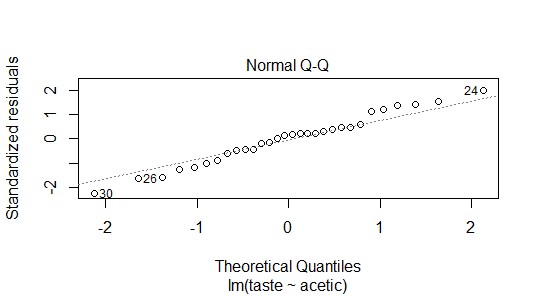
\includegraphics[width=.5\textwidth, height=60mm, keepaspectratio]{images/1155/1155qq.png}\par
	
	\begin{tabular}{cc}
		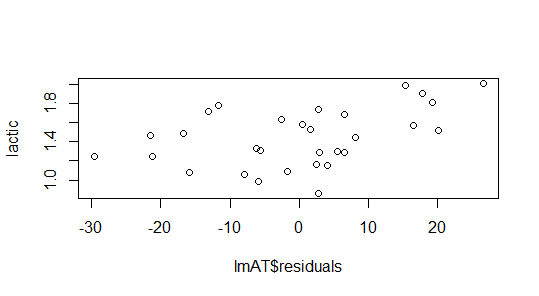
\includegraphics[width=.5\textwidth, height=60mm, keepaspectratio]{images/1155/1155_acetic_lactic_residuals_vs_lactic.png} & 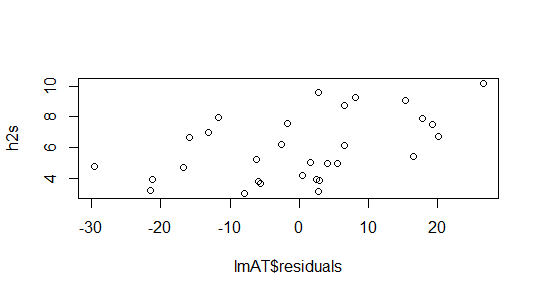
\includegraphics[width=.5\textwidth, height=60mm, keepaspectratio]{images/1155/1155_acetice_taste_residuals_vs_h2s.png}\\
	\end{tabular}\par
	
	Based on the above three graphs, the residuals seem to be relatively normal, and have some positive association with the other two variables.\par
	\end{center}\par
	
	
\newpage
\part{11.56}
	\begin{center}
	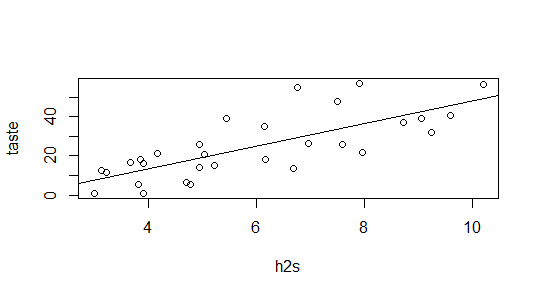
\includegraphics[width=.5\textwidth, height=60mm, keepaspectratio]{images/1156/h2s_taste_linear_regression.png}\par
	Summary\par
	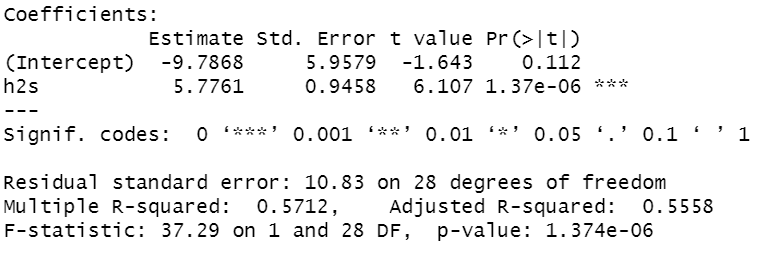
\includegraphics[width=.5\textwidth, height=60mm, keepaspectratio]{images/1156/taste_H2S_summary.PNG}\par
	H$_{0}: \beta_{1} = 0$, Taste and H2S are not related\par
	H$_{a}: \beta_{1} \ne 0$ Taste and H2S are related\par
	Since the p-value of $1.374*10^{-6} < 0.05$, we can reject H$_{0}$ and say that the model is statistically significant in that taste and H2S are related.\par
	
	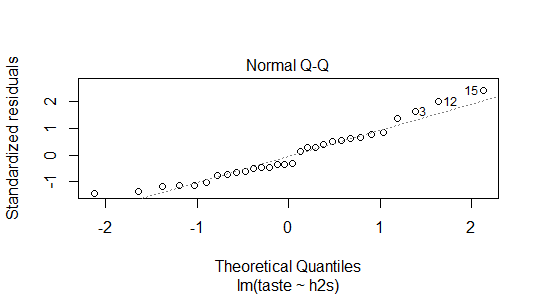
\includegraphics[width=.5\textwidth, height=60mm, keepaspectratio]{images/1156/1156qq.png}\par
	
	\begin{tabular}{cc}
		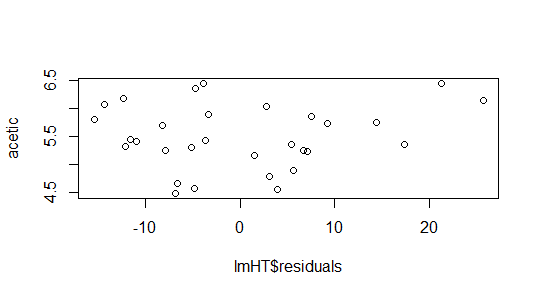
\includegraphics[width=.5\textwidth, height=60mm, keepaspectratio]{images/1156/H2S_taste_residuals_vs_acetic.png} & 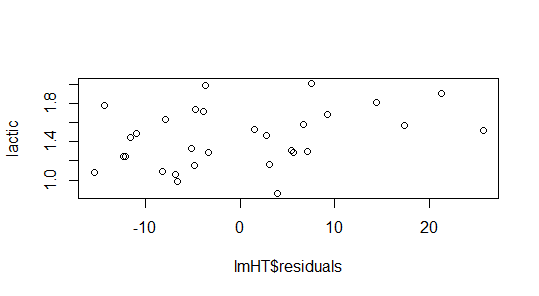
\includegraphics[width=.5\textwidth, height=60mm, keepaspectratio]{images/1156/H2S_taste_residuals_vs_lactic.png}\\
	\end{tabular}\par
	Based on the above three graphs, the residuals seem to be relatively normal, and no noticeable association with the other two variables.\par
	\end{center}\par
	
\newpage
\part{11.57}
	\begin{center}
	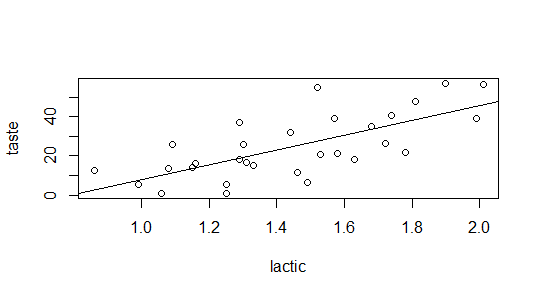
\includegraphics[width=.5\textwidth, height=60mm, keepaspectratio]{images/1157/taste_lactic_linear_regression.png}\par

	Summary\par
	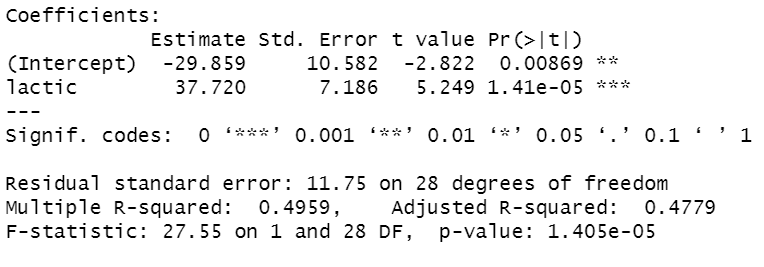
\includegraphics[width=.5\textwidth, height=60mm, keepaspectratio]{images/1157/lactic_taste_summary.PNG}\par
	H$_{0}: \beta_{1} = 0$, Taste and Lactic are not related\par
	H$_{a}: \beta_{1} \ne 0$ Taste and Lactic are related\par
	Since the p-value of $1.405*10^{-5} < 0.05$, we can reject H$_{0}$ and say that the model is statistically significant in that taste and lactic are related.\par
	
	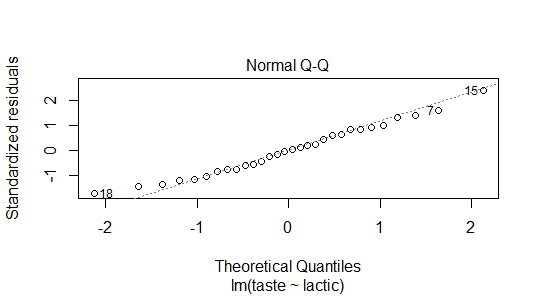
\includegraphics[width=.5\textwidth, height=60mm, keepaspectratio]{images/1157/1157qq.png}\par
	
	\begin{tabular}{cc}
		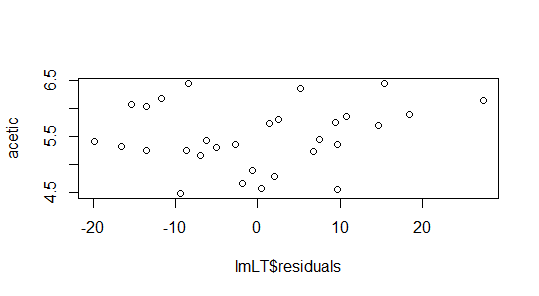
\includegraphics[width=.5\textwidth, height=60mm, keepaspectratio]{images/1157/lactic_taste_residuals_vs_acetic.png} & 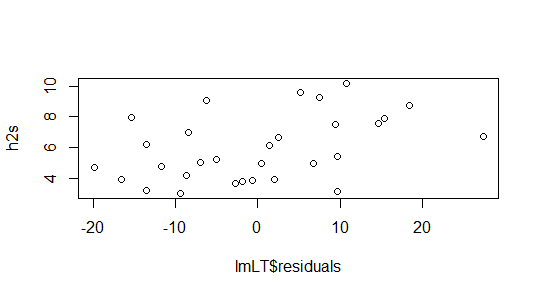
\includegraphics[width=.5\textwidth, height=60mm, keepaspectratio]{images/1157/lactic_taste_residuals_vs_h2s.png}\\
	\end{tabular}\par
	Based on the above three graphs, the residuals seem to be relatively normal, and no noticeable association with the other two variables.\par
	\end{center}\par

\newpage
\part{11.58}
	\begin{center}
	\begin{tabular}{lcccc}
		Regression Model & F Statistic & P-Value & R$^{2}$ & S\\
		Acetic & 12.11 & 0.001658 & 0.2771 & 13.82\\
		H2S & 37.29 & $1.37*10^{-6}$ & 0.5558 & 10.83\\
		Lactic & 27.55 & $1.41*10^{-5}$ &  0.4779 & 11.75\\
	\end{tabular}
	\end{center}\par
	
	$\hat{taste} = -61.499 + 15.648*acetic$\par
	$\hat{taste} = -9.7868 + 5.7761 * H2S$\par
	$\hat{taste} = -29.859 + 37.720 * lactic$\par
	
	The above three equations' intercepts are different because they are using three different explanatory variables.\par

\part{11.59}
	
	\begin{center}
	\begin{tabular}{cc}
		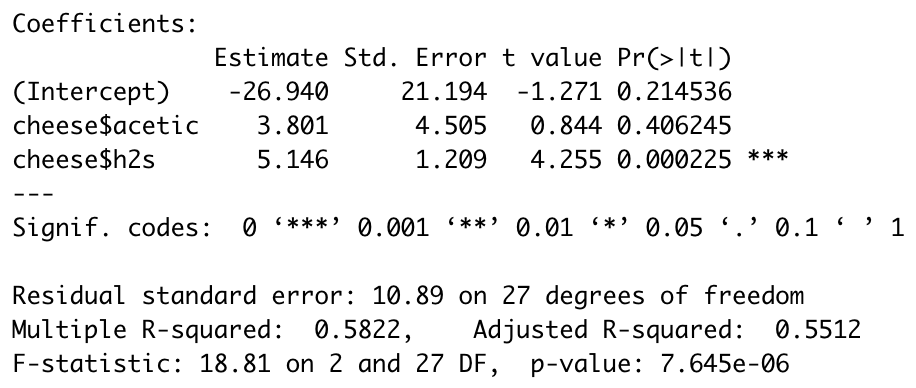
\includegraphics[width=.5\textwidth, height=60mm, keepaspectratio]{images/1159/1159summary.png} & 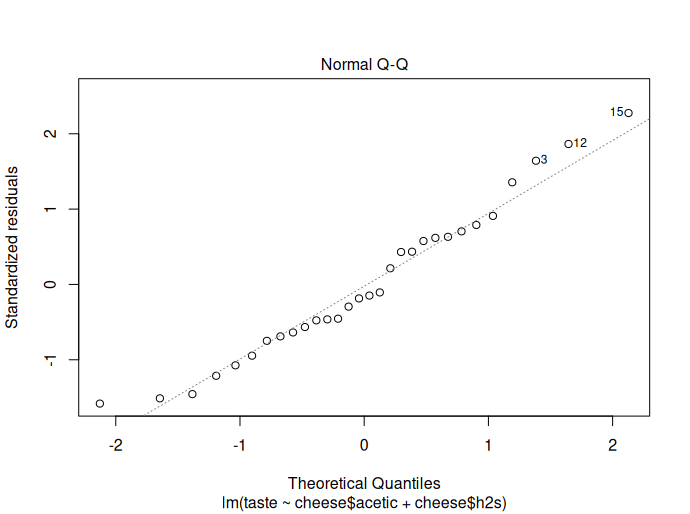
\includegraphics[width=.5\textwidth, height=60mm, keepaspectratio]{images/1159/1159qqplot.png}\\
	\end{tabular}
	\end{center}\par
	H$_{0}: \beta_{1} = 0$, Acetic and H2S are not related\par
	H$_{a}: \beta_{1} \ne 0$ Acetic and H2S are related\par
	Since the p-value of $7.645*10^{-6} < 0.05$, we can reject H$_{0}$ and say that the model is statistically significant in that acetic and H2S are related.\par
	In terms of the residual, it appears to be relatively normal.\par
	This model does not seem to be better than the other model containing H2S. Since acetic and H2S are correlated, acetic doesn't add any significance.\par

\newpage
\part{11.60}

	\begin{center}
	\begin{tabular}{cc}
		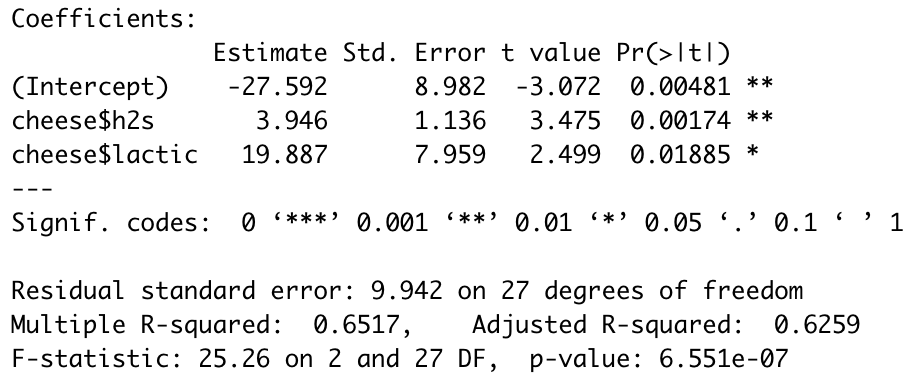
\includegraphics[width=.5\textwidth, height=60mm, keepaspectratio]{images/1160/1160summary.png} & 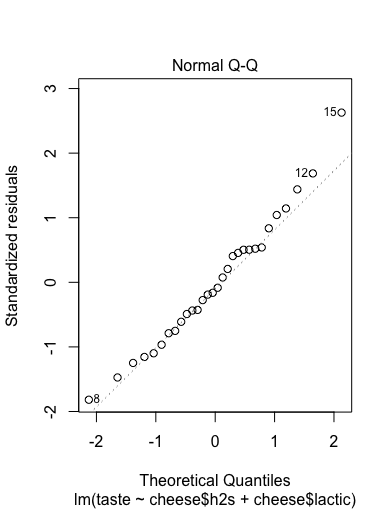
\includegraphics[width=.5\textwidth, height=60mm, keepaspectratio]{images/1160/QQplot.png}\\
	\end{tabular}
	\end{center}\par
	H$_{0}: \beta_{1} = 0$, H2S and Lactic are not related\par
	H$_{a}: \beta_{1} \ne 0$ H2S and Lactic are related\par
	Since the p-value of $6.551*10^{-7} < 0.05$, we can reject H$_{0}$ and say that the model is statistically significant in that H2S and lactic are related.\par
	The residual appear to be relatively normal. The p-value is significantly lower in comparison to the previous two variables alone, therefore, it is more significant and a better model.\par

\part{11.61}

	\begin{center}
	\begin{tabular}{cc}
		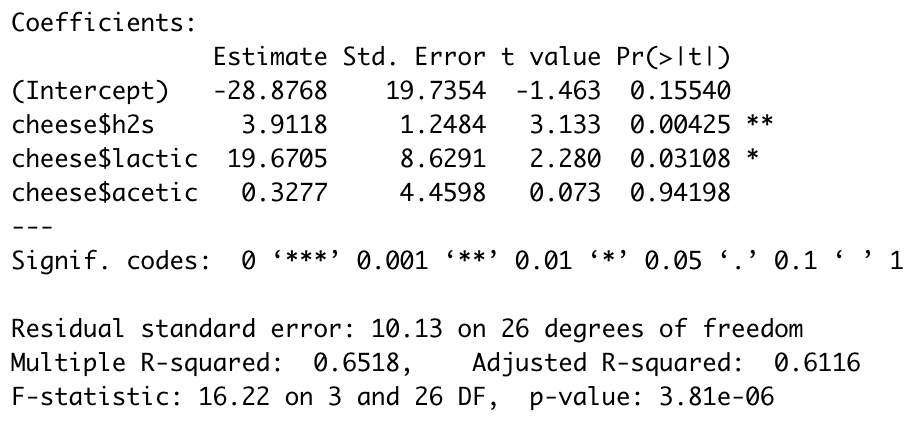
\includegraphics[width=.5\textwidth, height=60mm, keepaspectratio]{images/1161/1161summary.png} & 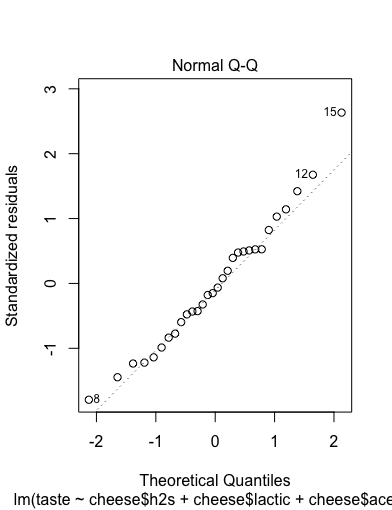
\includegraphics[width=.5\textwidth, height=60mm, keepaspectratio]{images/1161/qqplot.png}\\
	\end{tabular}
	\end{center}\par
	H$_{0}: \beta_{1} = 0$, H2S, Lactic, and Acetic are not related\par
	H$_{a}: \beta_{1} \ne 0$, H2S, Lactic, and Acetic are related\par
	Since the p-value of $3.81*10^{-6} < 0.05$, we can reject H$_{0}$ and say that the model is statistically significant in that H2S, lactic, and acetic are related.\par
	It would appear that the multiple regression model combining H2S and lactic is the best because it has the smallest p-value and is statistically the most significant.\par
	
\end{document}